\section{Memory model and memory injections}\label{sec:compcert-mem}

All intermediate languages in \compcert\ use the same memory model \cite{Leroy-Blazy-memory-model}. This is a key feature of the CompCert's proof of correctness, since it facilitates reasoning about how the compiler lays out stack frames in memory. In this section we briefly describe the memory model and the \emph{memory injections} which describe the evolution of the memories (particularly stack frames) through compilation.


\begin{figure}
$$\begin{array}{rccl} 
&\text{block}& ::= & \mathbb{N} \\
\text{Blocks} &  b & ::= &\text{block} \\
\text{Offsets} & ofs & ::= & \mathbb{Z} \\
\text{Values} & v & ::= & \text{Vundef} \ |\  \text{Vint}\ n \ |\  \text{Vfloat}\ n \ |\  \text{Vptr}\ b\ ofs \\
\text{mem} & m & \in & \mathbb{N} \rightarrow \text{option} (\mathbb{N} * \mathbb{Z}) \\
\text{perm} & p & ::= & \text{None} \ |\  \text{Nonempty} \ |\  \text{Readable} \ |\  \text{Writable} \ |\  \text{Freeable} \\
\text{Max perm} & \text{Max} & \in & \text{mem}\rightarrow (\text{block} * \mathbb{Z}) \rightarrow \text{Perm} \\
\text{Cur perm} & \text{Cur} & \in & \text{mem}\rightarrow (\text{block} * \mathbb{Z}) \rightarrow \text{Perm} \\
\text{injection}& j& \in & \text{block} \rightarrow \text{option} (\text{block} * \mathbb{Z})\\
\end{array}$$
\caption{\compcert\ memory model.}
\end{figure}
CompCert's memory is represented by a two dimensional array of bytes, indexed by a block reference and an integer offset. Each single block is a one dimensional array that can be used differently for each intermediate language; in Clight, every stack-allocated variable is in a separate block while in Mach every stackframe sits in a single block. The bytes in each location are represented by abstract values such as integers, floats, pointers; or undefined, if its location has not been initialized. 
  
Every location in memory is also outfitted with permissions that regulate how a program can interact with memory. These permissions are cumulative, so each one grants the capabilities of all the permissions below:

\begin{tabular}{rl} 
Freeable: & can free the location \\
Writable: & can write to the location\\
Readable: & can read to the location\\
Nonempty: & can only compare pointers to the given location\\
None: & Can't interact with the location\\
\end{tabular}

For example, a program may only free a piece of memory if it has \Coqcode{Freeable} permission of that location; but it can read any location where it has at least \Coqcode{Readable} permission. 
It is intended that a thread may gain or lose permissions to a location by doing synchronizations such as acquire and release; to keep track of this, there is a \Coqcode{Cur} (current) permission at each address.  But to prove the correctness of a certain optimization (constant-folding the load of a global read-only variable), the semantics also has a \Coqcode{Max} permission at each address, above which Cur can never go.
For example, all global variables have at most \Coqcode{Writable Max}  permissions so they might change, but they can't be freed. \Coqcode{Cur} permissions represent local abilities of a module or thread. For example, a thread will have no permissions for variables in the stack of another thread, whose addresses are not taken. But no matter how much more \Coqcode{Cur} permission a thread gains by acquiring a lock (etc.), it can never go above the \Coqcode{Max} permission for the address.

The compiler must preserve the behavior of a compiling program, but it might reorder and change its accesses to memory; an optimization might swap two consecutive memory allocations, or it might add new ones during spilling. Even so, the memory can't change too much, lest it change the observable behavior of the program. In the CompCert memory model, the compiler can affect memory blocks by reordering them, deleting them, changing their internal offsets or even merging two of them. Leroy and Blazy \cite{Leroy-Blazy-memory-model} call these transformations \emph{memory injections} and, to prove memory-changing optimizations are correct, they show that the observable behavior of a correct program is invariant under memory injections. We will describe injections further below.

Most \compcert\ passes don't change the memory behavior of the program. For example, the phase Cshmgen simplifies control structures, but preserves all memory accesses. In that way, the executions of the program before and after the pass display the same memories at every point. These are \emph{equality passes}. Some passes might increase the size of a block by, for example, spilling variables to the stack, but won't reorder the blocks; we call these  \emph{extension passes} \autoref{fig:memtransforms}(b). Finally there are those that delete, reorder and merge blocks, such as the Csharpminor to Cminor pass which merges all stack-allocated variables into  single block (the stack block). These are the \emph{injection passes}\ \autoref{fig:memtransforms}(a). All passes can be shown to be injections \cite{compcomp}, but it is much easier to treat equality and extension phases as special cases. 

\begin{figure}
\begin{multicols}{2}
~~\raisebox{4ex}{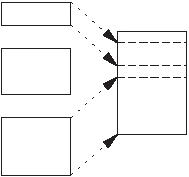
\includegraphics[height=90pt]{graphics/memfig3a.pdf}}

(a) Memory injection

\columnbreak
~~\raisebox{4ex}{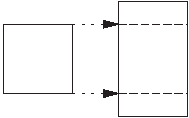
\includegraphics[height=90pt]{graphics/memfig3b.pdf}}

(b) Memory extension

%\columnbreak
%
%Equality diagram
%
%(c) Memory equality
\end{multicols}
\caption[Memory transformations of CompCert]{Memory transformations of CompCert. \cite{appel14:plcc}  }\label{fig:memtransforms}
\end{figure}

% More about injections
An injection is described by a mapping $j:$ \Coqcode{block -> option (block * Z)}, that determines if a block is mapped and, if so, to which block and with what offset. For example in the Csharpminor to Cminor pass, where local variables are coalesced into one stack block, each variable will be offset such that it doesn't overlap with the others as shown in \autoref{fig:memtransforms}(a). Beyond a permutation of memory, an injection induces relations between the source and target contents of memory and the permissions. We abuse the notation $\overset{j}{\hookrightarrow}$ to denote all these relations induced by injections, including several others we define in the following sections. 


\def\ofs{i} 

 \begin{figure}\centering
 %\begin{multicols}{2}

\fbox{
\begin{mathpar}
\inference{}{\mathsf{Vint}(n) \strinjarrow{j} \mathsf{Vint}(n)}
\and
\inference{}{\mathsf{Vfloat}(n) \strinjarrow{j} \mathsf{Vfloat}(n)}
\and
\inference{F(b_1) = \text{Some}\ (b_2, \delta) & \ofs_2 = \ofs_1 + \delta}{
\mathsf{Vptr}(b_1,\ofs_1) \strinjarrow{j} \mathsf{Vptr}(b_2,\ofs_2)}
\and
\inference{v_1 \strinjarrow{j} v_2}{v_1 \injarrow{j} v_2}
\and
\inference{}{\mathsf{Vundef}\injarrow{j} v_2}
\end{mathpar}
}
(a) Strong ($\strinjarrow{}$) and simpl ($\injarrow{}$) value injections.

%\columnbreak

\fbox{\begin{mathpar}
\inference{}{p \injarrow{j} p}
\and
\inference{}{\mathsf{None}\injarrow{j} \mathsf{Freeable}}
\end{mathpar}
}

(b) Permission injections

%\end{multicols}
\caption{Value and permission injections}\label{fig:valueinj_perminj}
\end{figure}

An injection imposes a relation between values before and after the compiler pass, as described in \autoref{fig:valueinj_perminj}(a). In the stronger injection, constants are preserved and pointers are renamed according to the injection. In the simpl injection, undefined values are also allowed to map to any concrete value because, in compiler passes such as register coalescing, uninitialized local variables, can map to initialized ones with concrete values. Similarly, the injection imposes a relation between permissions as shown in  \autoref{fig:valueinj_perminj}(b).


\begin{definition}[memory injection]\footnote{We omit a couple extra properties such as \emph{not overlapping} and \emph{memory alignment}.} Two memories $m_1$ and $m_2$ are \emph{injected} by $j$ ($m_1 \injarrow{j} m_2 $) if, for all locations $b_1$ mapped by $j \ b_1 = \text{Some}\ (b_2, \text{ofs})$ :
\begin{itemize}
\item Permissions are injected on all offsets $x$: 
$$\text{Max}\ m_1\ (b_1,\ x)  \injarrow{j} \text{Max}\ m_2\ (b_2,\ x + \text{ofs}) \ \ \ \text{and}$$ $$\text{Cur}\ m_1\ (b_1,\ x)  \injarrow{j} \text{Cur}\ m_2 (b_2,\ x + \text{ofs})$$

\item Values are injected on all visible offsets $x$: 
$$\text{Cur}\ m_1\ (b_1,\ x)  \geq \text{Readable} \rightarrow m_1\ (b_1,\ x)  \injarrow{j} m_2\ (b_2,\ x + \text{ofs})$$

\item Only allocated blocks are mapped and the image of mapped blocks don't overlap.

\item \Coqcode{mi_representable} and \Coqcode{mi_perm_inv} \cite{appel14:plcc}  

\end{itemize}
\end{definition}







   
